% Nallino, Part II p. 253: digressions and obliquities of the points of the epicycle, redrawn from the print at the
% size of the print. The coordinates are those of a 400 dpi render of the figure (crop from x 355 pt, y 436 pt of the
% master page; y downward). The epicycle has its centre in H; GHE is the line to the Earth E, ED the tangent, EFN a
% secant; I, K, M are the feet of the perpendiculars from F, D, N on the plane of the ecliptic. Dashed as on the
% print: NM, ME (through I), IF, DK and KE.
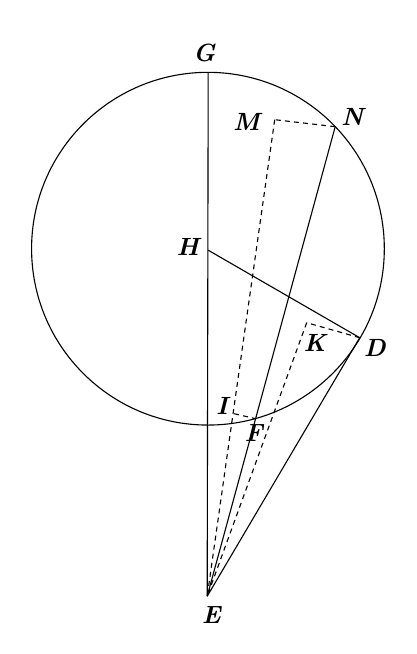
\begin{tikzpicture}[x=0.0635mm,y=-0.0635mm,line width=0.4pt,every node/.style={font=\bfseries\itshape\small,inner sep=1pt}]
\path (5,15);
\coordinate (H) at (366,460);
\coordinate (E) at (364,1152);
\coordinate (D) at (669,635);
\coordinate (N) at (620,213);
\coordinate (F) at (461,797);
\coordinate (M) at (499,199);
\coordinate (I) at (418,787);
\coordinate (K) at (563,605);
\draw (365.5,457) circle[radius=352.7];
\draw (366,104.3) -- (E);
\draw (H) -- (D);
\draw (D) -- (E);
\draw (N) -- (E);
\begin{scope}[dash pattern=on 1.8pt off 1.5pt]
\draw (N) -- (M);
\draw (M) -- (E);
\draw (I) -- (F);
\draw (D) -- (K);
\draw (K) -- (E);
\end{scope}
\node at (358,65.5) {G};
\node at (442.5,204) {M};
\node at (654,193.5) {N};
\node at (325,453.5) {H};
\node at (579,646) {K};
\node at (699,655) {D};
\node at (393.5,771) {I};
\node at (457,826) {F};
\node at (372,1189) {E};
\end{tikzpicture}
